/%% abtex2-modelo-projeto-pesquisa.tex, v-1 PFC 1 2016
%% Copyright 2012-2015 by abnTeX2 group at http://www.abntex.net.br/ 
%%
%% This work consists of the files abntex2-modelo-projeto-pesquisa.tex
%% and abntex2-modelo-references.bib
%%

% ------------------------------------------------------------------------
% ------------------------------------------------------------------------
% abnTeX2: Modelo de Projeto de pesquisa em conformidade com 
% ABNT NBR 15287:2011 Informação e documentação - Projeto de pesquisa -
% Apresentação 
% ------------------------------------------------------------------------ 
% ------------------------------------------------------------------------

\documentclass[
	% -- opções da classe memoir --
	12pt,				% tamanho da fonte
	openright,			% capítulos começam em pág ímpar (insere página vazia caso preciso)
	oneside,
    %twoside,			% para impressão em verso e anverso. Oposto a oneside
	a4paper,			% tamanho do papel. 
	% -- opções da classe abntex2 --
	%chapter=TITLE,		% títulos de capítulos convertidos em letras maiúsculas
	%section=TITLE,		% títulos de seções convertidos em letras maiúsculas
	%subsection=TITLE,	% títulos de subseções convertidos em letras maiúsculas
	%subsubsection=TITLE,% títulos de subsubseções convertidos em letras maiúsculas
	% -- opções do pacote babel --
	english,			% idioma adicional para hifenização
	french,				% idioma adicional para hifenização
	spanish,			% idioma adicional para hifenização
	brazil,				% o último idioma é o principal do documento
	]{abntex2}

% ---
% PACOTES
% ---

% ---
% Pacotes fundamentais 
% ---
\usepackage{lmodern}			% Usa a fonte Latin Modern
\usepackage[T1]{fontenc}		% Selecao de codigos de fonte.
\usepackage[utf8]{inputenc}		% Codificacao do documento (conversão automática dos acentos)
\usepackage{indentfirst}		% Indenta o primeiro parágrafo de cada seção.
\usepackage{color}				% Controle das cores
\usepackage{graphicx}			% Inclusão de gráficos
\usepackage{microtype} 			% para melhorias de justificação
\usepackage{verbatim}           % comentar em bloco

% ---

% ---
% Pacotes adicionais, usados apenas no âmbito do Modelo Canônico do abnteX2
% ---
\usepackage{lipsum}				% para geração de dummy text
% ---

% ---
% Pacotes de citações
% ---
\usepackage[brazilian,hyperpageref]{backref}	 % Paginas com as citações na bibl
\usepackage[alf]{abntex2cite}	% Citações padrão ABNT

% --- 
% CONFIGURAÇÕES DE PACOTES
% --- 

% ---
% Configurações do pacote backref
% Usado sem a opção hyperpageref de backref
\renewcommand{\backrefpagesname}{Citado na(s) página(s):~}
% Texto padrão antes do número das páginas
\renewcommand{\backref}{}
% Define os textos da citação
\renewcommand*{\backrefalt}[4]{
	\ifcase #1 %
		Nenhuma citação no texto.%
	\or
		Citado na página #2.%
	\else
		Citado #1 vezes nas páginas #2.%
	\fi}%
% ---

% ---
% Informações de dados para CAPA e FOLHA DE ROSTO
% ---
\titulo{Uso de Redes Neurais Artificiais na Predição do Risco de Reprovação de Alunos na Educação de Computação}
\autor{Lucas Rodrigues Costa} % do Curso de Ciências da Computação}
\local{Jataí-GO}
\data{2019}
\tipotrabalho{Projeto de Pesquisa (Graduação)}
% O preambulo deve conter o tipo do trabalho, o objetivo, 
% o nome da instituição e a área de concentração 
\preambulo{Projeto de Pesquisa apresentado ao curso de Bacharelado em Ciências da Computação, como requisito para obtenção do grau final na disciplina de Projeto Final de Curso 1.}

\orientador {Prof. Me. Esdras Lins Bispo Jr.}

\instituicao{Universidade Federal de Goiás - Regional Jataí}

% ---

% ---
% Configurações de aparência do PDF final

% alterando o aspecto da cor azul
\definecolor{blue}{RGB}{41,5,195}

% informações do PDF
\makeatletter
\hypersetup{
     	%pagebackref=true,
		pdftitle={\@title}, 
		pdfauthor={\@author},
    	pdfsubject={\imprimirpreambulo},
	    pdfcreator={LaTeX with abnTeX2},
		pdfkeywords={abnt}{latex}{abntex}{abntex2}{projeto de pesquisa}, 
		colorlinks=true,       		% false: boxed links; true: colored links
    	linkcolor=blue,          	% color of internal links
    	citecolor=blue,        		% color of links to bibliography
    	filecolor=magenta,      		% color of file links
		urlcolor=blue,
		bookmarksdepth=4
}
\makeatother
% --- 

% --- 
% Espaçamentos entre linhas e parágrafos 
% --- 

% O tamanho do parágrafo é dado por:
\setlength{\parindent}{1.3cm}

% Controle do espaçamento entre um parágrafo e outro:
\setlength{\parskip}{0.2cm}  % tente também \onelineskip

% ---
% compila o indice
% ---
\makeindex
% ---

% ----
% Início do documento
% ----
\begin{document}

% Seleciona o idioma do documento (conforme pacotes do babel)
%\selectlanguage{english}
\selectlanguage{brazil}

% Retira espaço extra obsoleto entre as frases.
\frenchspacing 

% ----------------------------------------------------------
% ELEMENTOS PRÉ-TEXTUAIS
% ----------------------------------------------------------
% \pretextual

% ---
% Capa
% ---
\imprimircapa
% ---

% ---
% Folha de rosto
% ---
\imprimirfolhaderosto
% ---

% ---
% NOTA DA ABNT NBR 15287:2011, p. 4:
%  ``Se exigido pela entidade, apresentar os dados curriculares do autor em
%     folha ou página distinta após a folha de rosto.''
% ---

% ---
% inserir lista de ilustrações
% ---
\pdfbookmark[0]{\listfigurename}{lof}
\listoffigures*
\cleardoublepage
% ---

% ---
% inserir lista de tabelas
% ---
\pdfbookmark[0]{\listtablename}{lot}
\listoftables*
\cleardoublepage
% ---

% ---
% inserir lista de abreviaturas e siglas
% ---
\begin{siglas}
  %\item[ABNT] Associação Brasileira de Normas Técnicas
  %\item[abnTeX] ABsurdas Normas para TeX
  \item[ARL - Análise de Regressão Linear]
  \item[IpC - Instrução pelos Colegas]
  \item[INEP - Instituto Nacional de Estudos e Pesquisas Educacionais Anísio Teixeira]
  \item[MEC - Ministério da Educação]
  \item[SIGCSE - Special Interest Group onComputer Science Education]
  \item[WEI - Workshop sobre Educação em Computação]


\end{siglas}
% ---

% ---
% inserir lista de símbolos
% ---
\begin{simbolos}
  \item[$ \Gamma $] Letra grega Gama
  \item[$ \Lambda $] Lambda
  \item[$ \zeta $] Letra grega minúscula zeta
  \item[$ \in $] Pertence
\end{simbolos}
% ---

% ---
% inserir o sumario
% ---
\pdfbookmark[0]{\contentsname}{toc}
\tableofcontents*
\cleardoublepage
% ---


% ----------------------------------------------------------
% ELEMENTOS TEXTUAIS
% ----------------------------------------------------------
\textual

% ----------------------------------------------------------
% Introdução
% ----------------------------------------------------------
\chapter*[Introdução]{Introdução}
\addcontentsline{toc}{chapter}{Introdução}

\begin{comment}{
%==========================================================================================
{\color{red}[MODELO]
A INTRODUÇÃO é apresentada em forma de um texto “corrido”, ou seja, de uma única redação em que deverão ser apresentados os elementos: tema (objeto de estudo, problema e área/sub-área); objetivos (geral e específicos) e justificativas.

Contextualiza-se o tema segundo o Marco Teórico/Estado da Arte que sustentará o desenvolvimento da pesquisa. Há que se esclarecer os limites para o seu desenvolvimento, a JUSTIFICATIVA da investigação por meio de uma REVISÃO BIBLIOGRÁFICA, em que se faz referência a estudos e pesquisas já realizados sobre o assunto em questão. O TEMA da pesquisa define o objeto de estudo a ser tratado. Pode equivaler ou não ao título do projeto ou da pesquisa. Deve ter um significado preciso. Já o PROBLEMA deve ser ainda mais específico e detalhado que o objeto de estudo. O problema também deve ser pautado em um levantamento bibliográfico. O problema, formulado como pergunta, deve ser associado ao marco teórico da investigação a ser feita e as demandas institucionais e sociais. Além disso, deve ser completo, ou seja, conter as variáveis necessárias e esclarecedoras da investigação. 
A revisão bibliográfica, para justificar a pesquisa, pode ser feita, optando-se por um dos seguintes argumentos:
\begin{enumerate}
\item o pesquisador demonstra a análise incompleta ou insuficiente acerca do objeto de estudo;
\item por meio da literatura selecionada, o estudioso demonstra contradições entre os autores em relação ao problema enunciado;
\item o estudioso deseja colocar em xeque as conclusões encontradas sobre o objeto de estudo;
\item o pesquisador necessita retestar os resultados já obtidos em outras investigações.
\item a área carece de inovações, adequações, melhorias ou contribuições acerca de uma tema.
\item a área pode ser solução para melhoria ou resolução de problemas de outras áreas afins ou não.
\end{enumerate}

Os OBJETIVOS são as metas conceituais a serem alcançadas com a realização do trabalho, por meio de verbos no infinitivo, como: demonstrar, identificar, observar, analisar, comparar. A melhor forma de destacá-los é dividi-los em geral / específicos. O GERAL deve se referir ao produto que se deseja obter com a investigação. 

Já OBJETIVOS ESPECÍFICOS (devem conter, no mínimo, três) possuem natureza operacional, isto é, referem-se a procedimentos que deverão ser cumpridos para que o objetivo geral seja atingido, confirmando ou não a hipótese enunciada.

É importante lembrar ao definir os objetivos específicos que os mesmos devem estar coerentes com a metodologia do trabalho (passos necessários para atingir os objetivos) e com o cronograma (tempo/prazo de execução do trabalho).
Para enriquecer a seção de Objetivos (geral e específicos) é salutar apresentar estratégias para atingir os objetivos e quantificar metas a serem alcançadas.
	
    A HIPÓTESE é a tentativa de explicação ou solução do problema enunciado, expressa na forma de sentença afirmativa. Deve também estar de acordo com o Estado da Arte/Marco Teórico definido. Trata-se de um ato criativo. Deve possuir clareza conceitual, referir-se a conceitos passíveis de verificação (empírica). A \autoref{metodo_cient} ilustra quais são as fases de uma pesquisa.

\begin{figure}[!htb]
    \centering
    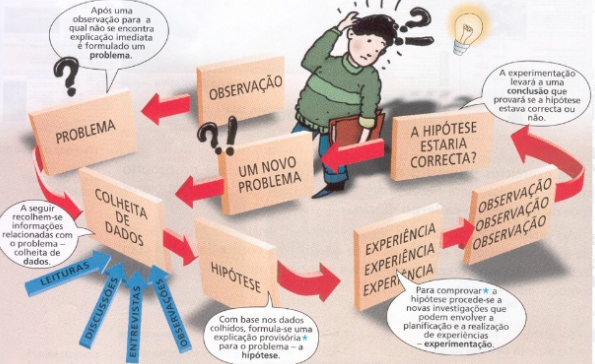
\includegraphics[scale=0.70]{metodo.png}
    \caption{Fases de uma pesquisa}
    \label{metodo_cient}
\end{figure}

Uma lista completa das normas
observadas pelo \abnTeX\ é apresentada em \citeonline{abntex2classe}.



Este documento deve ser utilizado como complemento dos manuais do \abnTeX\ 
\cite{abntex2classe,abntex2cite,abntex2cite-alf}. Consulte \citeonline{abntex2modelo} para obter
exemplos e informações adicionais de uso de \abnTeX\ e de \LaTeX. }
}
%===========================================================================================

\end{comment}

%Objeto de estudo
%Problema
%Área
%Objetivos
    % - Geral
    % - Específico
%Justificativa

%Ideias principais, da maior pra menor

% 1 - Afirmação geral sobre a área: Educação de computação
% 2 - Problema da área: Avaliação, identificação prévia de alunos em situação de risco
% 3 - Como os autores da área vem resolvendo esse problema
    % 3.1 - Para tentar resolver esse problema, esse autor fez isso.
    % 3.2 - Para tentar resolver, esse autor fez isso.
    % 3.3 - Para...
% É possível que essas soluções apresentem lacunas. Cewrtamente, usar no Brasil
% A proposta do meu trabalho é: Atacar essa lacuna diante do que já existe

% 1

A educação de Ciência da Computação é uma área emergente e assunto amplamente discutido pela comunidade acadêmica brasileira e internacional \cite{fincher2005mapping}. No contexto brasileiro, o Workshop sobre Educação em Computação (WEI) tem sido um dos principais fóruns para esta discussão. O Simpósio SIGCSE (\textit{Special Interest Group on Computer Science Education}) é um dos maiores eventos, em âmbito internacional, na área. {\color{red}[TERMINAR]}

%Problema
Muitos alunos ingressantes em Computação, apresentam dificuldades na aprendizagem, assim como em outras áreas de exatas. Em virtude destas dificuldades, alguns alunos não alcançam um desempenho satisfatório e reprovam. Estas reprovações podem ter, dentre outros fatores, forte influência em uma eventual evasão \cite{evasaoMatheus2014}. Segundo dados do Censo da Educação Superior de 2017 \cite{Inep2017}, publicado pelo Instituto Nacional de Estudos e Pesquisas Educacionais Anísio Teixeira (INEP) do Ministério da Educação (MEC), a taxa de evasão do Bacharelado em Ciência da Computação, nas universidades públicas e privadas de todo o Brasil, alcançou cerca de 60,2\%, enquanto a taxa geral - média dentre todos os cursos - ficou em torno dos 26\%.

Um dos problemas na educação de computação está na avaliação de aprendizagem dos alunos, tendo como ponto de interesse
%Justificativa
%Muitas vezes os ingressantes não conseguem acompanhar o fluxo de estudos, têm baixo desempenho e assim acabam evadindo ou reprovando nas matérias introdutórias do curso.
%Um dos pontos está no interesse 
a identificação prévia dos alunos que apresentam maior dificuldade na disciplina e, assim, com maior risco de reprovação.\cite{martins2012assistente}. {\color{red}[TERMINAR]}

Alguns autores propuseram métodos para solucionar esse problema. Podemos citar alguns autores e seus trabalhos, que abordaram modelos preditivos quanto a situação dos alunos.

% 1 - Lightweight, Early Identification of At-Risk CS1 Students - abstract: "Uso de Clicker para identificar riscos" [CI];
Liao et. al. \cite{liao2016lightweight} utilizou o modelo de \textbf{ARL (Análise de Regressão Linear)}, para fazer a análise dos dados gerados através do uso do IpC (Instrução pelos Colegas)\footnote[1]{Do inglês, \textit{Peer Instruction} (PI)} juntamente com o \textit{Clicker} pelos alunos para tentar identificar alunos com tendência a baixo desempenho na disciplina, baseado nas respostas dadas nas 3 primeiras semanas de aulas. O modelo proposto alcançou, aproximadamente, 70\% de acurácia na identificação de alunos com risco de reprovação, com 17\% dos alunos reprovados sendo erroneamente classificados - "falsos negativos"\footnote[2]{"Falsos negativos": Alunos previamente classificados como integrantes do "Grupo de risco", mas que, ao final da disciplina, obtiveram êxito.}.

% 11 - Importance of early performance in CS1: two conflicting assessment stories - abstract: "Uso de PI para relação entre desempenho inicial do curso e sucesso no curso" [CI];
Porter e Zingaro \cite{porter2014importance} usam os dados coletados durante o uso do IpC, além dos dados de provas, para explorar as relações entre as avaliações e o desempenho em sala de aula no final do prazo. Para examinar a relação entre as notas dos alunos em avaliações diferentes, foi utilizada a \textbf{Correlação de Pearson}.

% 28 - Automatically Classifying Students in Need of Support by Detecting Changes in Programming Behaviour - abstract: 
Estay, Keuning, Coady \cite{estey2017automatically} propuseram um método preditor que detecta, com 81\% de precisão, os estudantes em situação de risco de reprovação na disciplina de programação. O estudo foi desenhado para avaliar a aprendizagem do aluno através da detecção de \textbf{mudanças no comportamento} de programação ao longo do tempo. 

 Uma outra proposta é o uso do \textbf{modelo PreSS} que usa fatores comparativos - como a eficiência de programação, a habilidade matemática  e as horas dedicadas em exercícios - para auxiliar a identificação do alunos em risco de reprovação \cite{quille2018}. Existem até ferramentas capazes de realizarem capturas de telas, que exibem código-fonte, para auxiliar na identificação das dificuldades apresentadas pelos alunos usando \textbf{aprendizado de máquina}\cite{ahadi2016early}.
 
%Objetivos Geral/Específico
O objetivo geral deste trabalho é prever o desempenho acadêmico dos alunos, ainda no inicio da disciplina, identificando os que estejam no "grupo de risco"\footnote{Alunos em risco: Os alunos em situação de risco são aqueles que estão propensos a não concluir um curso, seja por insuficiência de presença ou de desempenho. \cite{da2014alunos}}, possibilitando ao professor intervir. Este projeto de pesquisa tem como objetivo específico propor um método, que preencha lacuna(s) deixada(s) pelos trabalhos supracitados e seus métodos preditivos, além de suprir a falta de relatos de casos no Brasil, apresentando um estudo de caso na disciplina de Interface Humano-Computador, no curso de Ciência da Computação da Universidade Federal de Goiás - Regional Jataí/Universidade Federal de Jataí, com os dados coletados durante o uso da plataforma de Aprendizagem Baseado em Jogos, "Kahoot!".

{\color{red}[OBJETO DE ESTUDO]}
%Objeto de estudo
%Esta pesquisa tem como objeto de estudo a Avaliação da Aprendizagem de Ciência da Computação. e o problema de avaliação e identificação preditiva do desempenho acadêmico de alunos, com base os dados coletados dos alunos em avaliações formativas no inicio da disciplina.

% ----------------------------------------------------------
% Elementos Textuais
% ----------------------------------------------------------
\chapter{Referencial Teórico}
Para melhor compreensão do texto, é importante a definição de alguns conceitos usados durante o mesmo. {\color{red}[MELhORAR]}

\begin{comment}{
{\color{red}[MODELO]
\index{elementos textuais} O Referencial Teórico é um seção dos elementos textuais. A norma ABNT NBR 15287:2011, p. 5, apresenta a
seguinte orientação quanto aos elementos textuais:

\begin{citacao}
O texto deve ser constituído de uma parte introdutória, na qual devem ser
expostos o tema do projeto, o problema a ser abordado, a(s) hipótese(s),
quando couber(em), bem como o(s) objetivo(s) a ser(em) atingido(s) e a(s)
justificativa(s). É necessário que sejam indicados o referencial teórico que
o embasa, a metodologia a ser utilizada, assim como os recursos e o cronograma
necessários à sua consecução.\citeonline{abntex2classe}
\end{citacao}, ,

Deve-se apresentar a fundamentação teórica que orientará o estudo. Recomenda-se situar a grande área, subárea e objeto de estudo. Se for necessário pode ser feito um resgate histórico para demonstrar a evolução da área. Faz-se necessário relatar o momento vivido pela área (Marco Teórico - Estado da Arte) geralmente intitulado de Trabalhos Relacionados.

O Referencial Teórico é considerado como um elemento de controle de toda a pesquisa, desde a problematização inicial. O pesquisador irá interpretar seu objeto de estudo de acordo com a concepção teórica de uma ou toda a obra de um autor ou de um objeto ou produto ou de um conjunto de autores (esta condução varia de acordo com cada área de conhecimento). Todas as etapas do projeto são definidas conforme esta escolha. Apresenta-se de modo aprofundado, respondendo quais os princípios, categorias, conceitos ou teorias fundamentam a pesquisa. Deve estar de acordo com o tema formulado e o raciocínio desenvolvido nas fases anteriores. 

}}
\end{comment}

\section{Educação de Computação}    

{\color{red} [PROCURAR MAIS]} 

Educação de computação é o resultado da fusão de, a princípio — Outras também estão envolvidas, como, por exemplo: Psicologia, engenharias, tecnologia, entre outras—, duas disciplinas: Educação e Computação. 

Educação é um processo que visa ao desenvolvimento físico, intelectual e moral do ser humano, através da aplicação de métodos próprios, com intuito de assegurar-lhe a integraçãoo social e formal da cidadania \cite{weiszflog1999michaelis}. Ciência da Computação é o estudo sistemático de algoritmo e estrutura de dados, i.e., o estudo do seu formalismo, desenvolvimento e aplicações. \cite{gibbs1986model}

O objetivo principal da pesquisa em Educação de Computação é o aperfeiçoamento do processo de ensino e apredizagem da Computação como ciência. \cite{holmboe2001research}

Fincher e Petre \cite{fincher2005mapping} identificam dez grandes áreas de interesse para pesquisadores em Educação de Computação. As dez áreas são: a compreensão do aluno, sistemas de animação/visualização/simulação, métodos de ensino, avaliação, tecnologia educacional, a transferência de prática profissional em sala de aula, a incorporação de um novo desenvolvimento e novas tecnologias na sala de aula, transferindo para o ensino à distância (“EaD” ou “\textit{e-learning}”), recrutamento e retenção de alunos, e finalmente, a construção da disciplina em à distância (“EaD” ou “\textit{e-learning}”), recrutamento e retenção de alunos, e finalmente, a construção da disciplina em à distância (“EaD” ou “\textit{e-learning}”), recrutamento e retenção de alunos, e finalmente, a construção da disciplina em à distância (“EaD” ou “\textit{e-learning}”), recrutamento e retenção de alunos, e finalmente, a construção da disciplina em si. 

{\color{red}[Melhorar frase]Este trabalho será em torno da área de avaliação.}

%Artigos ============================
{\color{red}LER}
\cite{da2014metodos}
\cite{perrenoud1999avaliaccao}

\section{Avaliação}
A avaliação é uma área ampla, que pode ser dividida em termos de tipos de avaliação, validade da avaliação e classificação automatizada. \cite{fincher2005mapping}

A avaliação pode ser definida como um processo sistemático de determinar a extensão em que os objetivos educacionais foram alcançados pelos alunos. O que se avalia são as metas de aprendizagem definidas e para as quais se caminhou durante todo um processo de aprendizagem levado a cabo pelo professor e pelo aluno \cite{domingos1981forma}

A avaliação da aprendizagem possibilita a tomada de decisão e a melhoria da qualidade de ensino, informando as ações em desenvolvimento e a necessidade de regulações constantes. \cite{kraemer2005avaliaccao}

A avaliação vista como uma etapa da aprendizagem passa a ser utilizada como um processo, isto é, na formação e construção do conhecimento levando a uma reflexão sobre as ações, gestos e pensamentos. Os processos formativos precisam ser avaliados em sua forma, efeito, método e evolução dos educandos. \cite{datrino2015avaliaccao}

Bloom e outros autores classificaram a avaliação em três tipos, sendo eles:
avaliação diagnóstica; avaliação formativa e avaliação somativa. \cite{bloom1983manual}

Os métodos avaliativos são de suma importância no processo de ensino-aprendizagem. Diversos autores demonstram os benefícios resultantes de uma boa avaliação durante as aprendizagens e conhecimentos adquiridos pelos discentes, porém precisam ser escolhidos e aplicados no cotidiano do aluno de forma a conduzi-lo à aprendizagem, obtendo assim resultados satisfatórios a partir de sua avaliação e evitando análises errôneas e estresse por parte dos educadores e educandos. \cite{da2014alunos}

\subsection{Avaliação diagnóstica}
Conhecer o aluno, seus gostos, seus hábitos e suas preferências, é o princípio base da avaliação diagnóstica. Dessa forma, assegura-se que o aluno esteja na turma correta e que o curso encontrese no nível adequado a ele. Nesta avaliação busca-se conhecer ideias e conhecimentos prévios do aluno \cite{masetto1994didatica}.

A avaliação diagnóstica visa verificar a existência, ou ausência, de
habilidades e conhecimentos pré‐estabelecidos, esta é uma ação que inicia o
processo avaliativo e verifica se os alunos dominam os pré‐requisitos necessários
para novas aprendizagens. \cite{bloom1983manual}

Segundo {\color{red}Haydt (2007)}, a partir de uma avaliação diagnóstica o docente constata se os seus alunos estão ou não preparados, se possuem domínio de pré–requisitos para adquirir novos conhecimentos. Portanto, a avaliação diagnóstica permite que o professor conheça seu aluno por um mecanismo de triagem e calibração

\subsection{Avaliação somativa}
Avaliação somativa é uma decisão que leva em conta a soma de um ou mais resultados e pode ser baseada numa só prova final {\color{red}(OLIVEIRA & CHADWICK, 2007)}.

Para {\color{red}Ballester et al. (2003)}, uma avaliação somativa possui uma função social de assegurar que as características dos estudantes respondam a determinadas exigências feitas pelo sistema.

De acordo com {\color{red}Haydt (2007)}, esse tipo de avaliação tem por princípio classificar os resultados de aprendizagem alcançados pelos alunos de acordo com os níveis de aproveitamento estabelecidos, adotando assim uma função classificatória.

A avaliação somativa pretende ajuizar o progresso realizado pelo aluno, no final de uma unidade de aprendizagem, no sentido de aferir resultados já recolhidos por avaliações do tipo formativo e obter indicadores que permitam aperfeiçoar o processo de ensino \cite{kraemer2005avaliaccao}.

\subsection{Avaliação formativa}
A idéia de avaliação formativa sistematiza o funcionamento, levando o professor a
observar mais metodicamente os alunos, a compreender melhor seus funcionamentos, de modo
a ajustar de maneira mais sistemática e individualizada suas intervenções pedagógicas e as
situações didáticas que propõe, tudo isso na expectativa de otimizar a aprendizagem: "A
avaliação formativa está portanto centrada essencial, direta e imediatamente sobre a gestão
das aprendizagens dos alunos (pelo professor e pelos interessados)". Essa concepção se situa
abertamente na perspectiva de uma regulação intencional, cuja intenção seria determinar ao
mesmo tempo o caminho já percorrido por cada um e aquele que resta a percorrer com vistas a
intervir para otimizar os processos de aprendizagem em curso. \cite{perrenoud1999avaliaccao}

A avaliação formativa pretende determinar a posição do aluno ao
longo de uma unidade de ensino, no sentido de identificar dificuldades
e de lhes dar solução {\color{red} [CITAR - Ribeiro, L (1989)]}

A avaliação formativa responde a uma concepção do ensino que considera que aprender é um longo processo, por meio do qual o aluno vai reestruturando seu conhecimento a partir das atividades que executa. Esse tipo de avaliação tem como finalidade fundamental a função ajustadora do processo de ensino-aprendizagem para possibilitar que os meios de formação respondam as características dos alunos. Pretende-se detectar os pontos fracos da aprendizagem, mais do que determinar quais os resultados obtidos com essa aprendizagem. \cite{jorba2003funccao}

\section{Inteligência Artificial}

\section{Aprendizado de Máquina}
\section{Redes Neurais Artificiais}
\section{Aprendizagem Baseada em jogos - Games-based Learning}
{\color{red}[Ler e procurar mais]}

Aprendizagem Baseada em jogos ou GBL pela sigla em inglês de \textit{Games-based Learning} foi definida por alguns autores. Segundo Tang, Hanneghan e El-Rhalibi \cite{tang2009introduction}, GBL faz referência a uma abordagem de aprendizagem inovadora derivada do uso de jogos de computador que tem valor educacional ou diferentes tipos de aplicação de software que usam jogos computacionais para ensino e educação. GBL's têm como finalidade o apoio à aprendizagem, a avaliação e análise de alunos e melhoria do ensino.

A aprendizagem baseada em jogos surge como uma alternativa de ensino que se adapta às características da pedagogia moderna na qual o estudante é um ator ativo \cite{monsalve2014aprendizagem}.

Com a aprendizagem baseada em jogos, se pretende equilibrar
entretenimento e difusão do conhecimento, motivando os estudantes a aprender
enquanto jogam \cite{monsalve2011teaching}.

\section{Kahoot!}
{\color{red}LER} \cite{diniz2018kahoot}

Kahoot! é uma plataforma de aprendizado baseada em jogos, usada como tecnologia educacional em escolas, universidades e outras instituições de ensino. Kahoot! foi fundada por Johan Brand, Jamie Brooker e MortenVersvik em um projeto conjunto com a Universidade Norueguesa de tecnologia e ciência. 

Seus jogos de aprendizado, "Kahoots", são \textit{quizzes}, perguntas de múltipla escolha, que permitem a criação de usuários e podem ser acessados por meio de um navegador da Web, telefone ou pelo aplicativo.

Kahoot! foi projetado para a aprendizagem social, com os alunos reunidos em torno de uma tela comum, como um quadro interativo, projetor ou um monitor de computador. O site também pode ser usado por meio de ferramentas de compartilhamento de tela, como Skype ou Google hangouts. Kahoot! pode ser usado para revisar o conhecimento dos alunos, para avaliação formativa, {\color{red}[]Citar o site <https://learninginnovation.duke.edu/blog/2015/07/kahoot-as-formative-assessment/>]} ou como uma pausa com as atividades tradicionais em sala de aula. 

A jogabilidade é simples; todos os jogadores se conectam usando um PIN de jogo gerado na tela comum e usam um dispositivo para responder a perguntas criadas pelo professor. As questões podem ter pontuações atribuídas, em relação ao acerto e ao tempo para resposta. Os pontos aparecem no placar depois de cada pergunta.

%Ler
{\color{red}LER}

    \cite{Souza:2017:GLB:3103028.3103054}\\
    \cite{pintor2014kahoot} No trabalho, o Kahoot! foi usado como base para o desenvolvimento de outro game educacional.
    
    \cite{chaiyo2017effect}\\
    \cite{abidin2017students}\\
    \cite{diniz2018kahoot}\\
    \cite{petri2016quiz}\\
    \cite{correia2017game}\\
    \cite{tobias2014game}\\
    \cite{wang2015wear}\\
    \cite{connolly2012systematic}\\
    \cite{backlund2013educational}
    
 Considerando que alguns fatores sociais e geográficos podem afetar a aplicação e a eficiência do uso desta ferramenta, faz-se necessário avaliá-la no contexto dos estudantes brasileiros.
 
 Em \cite{petri2016quiz}, o Kahoot! foi utilizado como um \textit{quiz} com perguntas sobre Gerenciamento de Projetos, disponibilizado para alunos dos cursos de Sistemas de
Informação e Ciência da Computação como forma de revisão de conteúdo. Os autores identificaram \textit{feedbacks} positivos nos resultados encontrados. Afirmaram também que o jogo educacional cumpriu com o seu objetivo de aprendizagem por proporcionar a revisão de conhecimentos de forma divertida e motivadora.

Para os autores \cite{abidin2017students}, a utilização do Kahoot! foi uma estratégia de motivação para os alunos de uma faculdade de Engenharia Elétrica ao cursarem uma disciplina de programação de computadores. O conteúdo apresentado no \textit{game} era relacionado a disciplina em questão e o objetivo era possibilitar aos alunos uma experiência atrativa para a aprendizagem, pois muitos deles perdiam o entusiamo ao estudarem programação de computadores. O resultado mostrou que a grande maioria dos alunos conseguiu melhorar sua  compreensão sobre a disciplina e também se mostraram mais engajados e motivados ao final do experimento.

Outro trabalho similar \cite{correia2017game} apresenta as opiniões de alunos de um programa de formação de professores (licenciatura e mestrado) sobre as vantagens e desvantagens da utilização do Kahoot! em sala de aula. Como vantagens percebidas estão a correção automática das questões e o \textit{feedback} em tempo real para os alunos e professores. Como desvantagens, foram identificados os seguintes fatores: numero limitado de caracteres tanto para o enunciado das questões quanto para as opções de respostas, além do tempo limitado de resposta.

%Artigo WEI
O principal objetivo do estudo foi identificar percepções acadêmico. Objetivos mais específicos consistiram em verificar a aceitação da mesma com base em algumas perspectivas além de elucidar as vantagens e desvantagens da sua utilização. Os resultados foram bastantes satisfatórios no que diz respeito a aceitação da ferramenta no contexto educacional, pelo seu caráter divertido, interessante e dinâmico os quais remetem a aprendizagem, conforme a percepção dos alunos. Também foi verificado que a sua utilização não causou efeito colateral nas respostas dos participantes.

Kahoot, mantém as mesmas utilidades que outros métodos de resposta rápida; especialmente os \textit{clickers}, mas sem todos os problemas técnicos e logísticos destes. \cite{pintor2014kahoot}

\section{Trabalhos Relacionados}
No decorrer dessa pesquisa foram encontrados alguns trabalhos que tratam de diferentes 

\cite{martins2012assistente}

\cite{gottardo2012previsao}

\cite{porter2014importance}

\cite{rodrigues2013modelo}

\cite{gotardo2013prediccao}
%===== Seção de Metodologia ==============

\chapter{Metodologia}

\begin{comment}{
%===========================================================================================
{\color{red}[MODELO]

\index{elementos textuais} A metodologia em um Projeto de Pesquisa preocupa-se muito mais com a classificação da pesquisa do que propriamente com a condução e execução do trabalho. Porém, o ideal é apresentar o detalhamento metodológico da pesquisa incluindo aspectos técnicos de execução específicos da área. Desta forma, o leitor ou avaliador poderá ter clareza do que será feito e como será feito. Lembrando que a execução metodológica deve estar alinhada com os objetivos específicos descritos na Introdução. 

\begin{enumerate}
\item
Tipo de Pesquisa: Pode-se fazer pesquisa bibliográfica, documental, experimental, estudo de caso e outros tipos. Na área tecnológica, a maioria dos trabalhos é classificada como experimental (quando há um protótipo desenvolvido) e estudo de caso (se situação problemática é relacionada à uma empresa).

\item
	Universo, População e Amostragem:
Deve-se identificar a população da qual você está retirando a sua amostra. Por exemplo, se sua pesquisa envolve os alunos do curso de Sistemas de Informação, sua população é o número total destes alunos, por exemplo 250 alunos. Se você decide então fazer uma amostragem, digamos de 10\%, então sua amostra para fins de sua pesquisa será de 25 alunos.
\item
	Coleta de Dados:
Deve-se indicar como irá operacionalizar a coleta os dados (questionários, check-lists, entrevistas, etc).
\item
	Análise e Interpretação dos Resultados:
Descreve-se neste item como será a análise dos resultados da pesquisa (se a pesquisa for qualitativa, as respostas podem ser interpretadas global ou individualmente, se a pesquisa for  quantitativa, você provavelmente irá utilizar a estatística descritiva ( média, mediana, moda, desvio padrão, tendência central) ou estatística inferencial (regressão linear bivariada, multivariada, etc).
\item
Os gêneros de pesquisa:
Em outra forma descritiva, a pesquisa também pode ser detalhada em termos de métodos obedecendo a classificação de natureza, objetivos, procedimentos, objeto e abordagem:
\begin{enumerate}
\item	Quanto à natureza
\begin{itemize}
\item Teórica - dita como conceitual, procura rever teorias ou formular novas idéias, parâmetros teórico-doutrinários, conceitos.
Metodológica - destina-se a redimensionar novos procedimentos de investigação, modos inovadores de construir ciência, transformação de metodologias tradicionais, introdução de novas técnicas de se conceber o objeto de estudo.
\item Empírica - dedica-se a mensurar a realidade; considera fatores sociais, políticos e econômicos na análise, em outras palavras, parte de constatações empíricas ou da realidade social para solucionar o problema da pesquisa; além disso, formula observações do real e propõe transformações do mesmo enquanto objeto de investigação.
\item Prática - embora semelhante à empírica, difere-se desta por se voltar a intervenções concretas no ambiente político, jurídico, ou sócio-cultural; transformações durante o trajeto da investigação ou análises que proponham novos rumos para a realidade social são os objetivos desse gênero.
\end{itemize}
\item
	Quanto aos objetivos
\begin{itemize}
\item Pesquisa exploratória
- Proporcionar maior familiaridade com o problema;
Levantamento bibliográfico ou entrevistas;
Pesquisa bibliográfica ou estudo de caso.
\item Pesquisa descritiva
- Fatos são observados, registrados, analisados, classificados e interpretados, sem interferência do pesquisador.
- Uso de técnicas padronizadas de coleta de dados (questionário e observação sistemática).
\item Pesquisa explicativa
- Identifica fatores determinantes para a ocorrência dos fenômenos.
- Ciências naturais – método experimental; ciências sociais – método observacional.
\end{itemize}
\item  Quanto aos procedimentos
\begin{itemize}
\item Pesquisa de campo – observação e coleta de dados diretamente no local da ocorrência dos fatos.
\item Pesquisa de fonte documental – pesquisa bibliográfica e documental.
\end{itemize}

\item
	Quanto ao objeto
\begin{itemize}
\item Pesquisa bibliográfica/documental – elaborada a partir de material já publicado (livros de quaisquer espécies, artigos de periódicos).
Pesquisa de laboratório – pesquisador procura refazer as condições de um fenômeno a ser estudado, para observá-lo sob controle.
\item Pesquisa de campo – pesquisador constrói um modelo da realidade, definindo formas de observá-la, formas de acesso a esse campo, os participantes e o campo da pesquisa.
\end{itemize}

\item
	Quanto à forma de abordagem
\begin{itemize}
\item Pesquisa quantitativa – traduz em números as opiniões e informações para serem classificadas e analisadas. Utilizam-se técnicas estatísticas.

\item Pesquisa qualitativa – é descritiva. As informações obtidas não podem ser quantificáveis. Os dados obtidos são analisados indutivamente. A interpretação dos fenômenos e a atribuição de significados são básicas no processo de pesquisa qualitativa. 
\end{itemize}
\end{enumerate}
\end{enumerate}
}
%===========================================================================================
}\end{comment}
Segundo  Yin  (2010)  são  os  estudos  de  caso  de  cunho  analítico  os  que  podem  proporcionar  significativo avanço no conhecimento real do contexto. Assim, essa abordagem se integra aos interesses da pesquisa, porque permite voltar o olhar para o processo de desistência por parte os  alunos  dos  seus  estudos. 
%===== Seção de Metodologia ==============


\chapter{Cronograma}

\index{elementos textuais}
O cronograma tem por objetivo prever as ações distribuídas de acordo com o tempo previsto de pesquisa. O cronograma deve estar alinhado com os objetivos específicos e com a metodologia. Nos objetivos específicos tem-se “o que vou fazer”, na metodologia, “como vou fazer” e no cronograma, “quando vou fazer”.

A  \autoref{tabela_cronog} apresenta o cronograma de execução da pesquisa. 

\begin{table}[!htb]
\centering
\caption{Cronograma de Atividades}
\label{tabela_cronog}
\begin{tabular}{@{}llll@{}}
\toprule
\textit{Atividades}                  & \textit{Mês}       & \textit{Ano}   \\ \midrule
Revisão Sistemática                  & Julho              & 2016      \\
Análise de Trabalhos Relacionados    & Agosto             & 2016      \\
Construção da Arquitetura            & Setembro           & 2016      \\
Implementação do Sistema             & Outubro            & 2016      \\
Avalição e Testes                    & Fevereiro          & 2017      \\
                                     &                    &           \\ \bottomrule
\end{tabular}
\end{table}




% ----------------------------------------------------------
% Capitulo com exemplos de comandos inseridos de arquivo externo 
% ----------------------------------------------------------

\include{abntex2-modelo-include-comandos}

% ---
% Finaliza a parte no bookmark do PDF
% para que se inicie o bookmark na raiz
% e adiciona espaço de parte no Sumário
% ---
\phantompart



% ----------------------------------------------------------
% ELEMENTOS PÓS-TEXTUAIS
% ----------------------------------------------------------
\postextual

% ----------------------------------------------------------
% Referências bibliográficas
% ----------------------------------------------------------
\bibliography{abntex2-modelo-references}

% ----------------------------------------------------------
% Glossário
% ----------------------------------------------------------
%
% Consulte o manual da classe abntex2 para orientações sobre o glossário.
%
%\glossary

% ----------------------------------------------------------
% Apêndices
% ----------------------------------------------------------

% ---
% Inicia os apêndices
% ---
\begin{apendicesenv}

% Imprime uma página indicando o início dos apêndices
\partapendices

% ----------------------------------------------------------
\chapter{Exemplo de um apêndice A}
% ----------------------------------------------------------



% ----------------------------------------------------------
\chapter{Exemplo de um apêndice B}
% ----------------------------------------------------------


\end{apendicesenv}
% ---


% ----------------------------------------------------------
% Anexos
% ----------------------------------------------------------

% ---
% Inicia os anexos
% ---
\begin{anexosenv}

% Imprime uma página indicando o início dos anexos
\partanexos

% ---
\chapter{Exemplo de um primeiro anexo}
% ---


% ---
\chapter{Exemplo de um segundo anexo}
% ---



% ---
\chapter{Exemplo de um terceiro anexo}
% ---



\end{anexosenv}

%---------------------------------------------------------------------
% INDICE REMISSIVO
%---------------------------------------------------------------------

\phantompart

\printindex


\end{document}
